% DO NOT COMPILE THIS FILE DIRECTLY!
% This is included by the other .tex files.

%\colorlet{punct}{red!60!black}
%\definecolor{background}{HTML}{EEEEEE}
%\definecolor{delim}{RGB}{20,105,176}
%\colorlet{numb}{magenta!60!black}

\lstdefinelanguage{json}{
    basicstyle=\ttfamily\footnotesize,
    numbers=left,
    numberstyle=\ttfamily\footnotesize,
    stepnumber=1,
    numbersep=8pt,
    showstringspaces=false,
    breaklines=true,
    frame=lines,
    backgroundcolor=\color{background},
    literate=
     *{0}{{{\color{numb}0}}}{1}
      {1}{{{\color{numb}1}}}{1}
      {2}{{{\color{numb}2}}}{1}
      {3}{{{\color{numb}3}}}{1}
      {4}{{{\color{numb}4}}}{1}
      {5}{{{\color{numb}5}}}{1}
      {6}{{{\color{numb}6}}}{1}
      {7}{{{\color{numb}7}}}{1}
      {8}{{{\color{numb}8}}}{1}
      {9}{{{\color{numb}9}}}{1}
      {:}{{{\color{punct}{:}}}}{1}
      {,}{{{\color{punct}{,}}}}{1}
      {\{}{{{\color{delim}{\{}}}}{1}
      {\}}{{{\color{delim}{\}}}}}{1}
      {[}{{{\color{delim}{[}}}}{1}
      {]}{{{\color{delim}{]}}}}{1},
}

\begin{frame}[t,plain]
\titlepage
\end{frame}

\begin{frame}
    \frametitle{MISP - VM}
    \begin{itemize}
    \item Credenciales
        \begin{itemize}
            \item MISP admin: admin@admin.test/admin
            \item SSH: misp/Password1234
        \end{itemize}
    \item Disponible para descargar aquí (VirtualBox and VMWare):
        \begin{itemize}
                \item \url{https://www.circl.lu/misp-images/latest/}
        \end{itemize}
    \end{itemize}
\end{frame}

\begin{frame}
    \frametitle{MISP - Uso Básico}
    Plan para esta parte de la capacitación
        \begin{itemize}
            \item Modelo de datos
            \item Visualizando datos
            \item Alta de datos
            \item Cooperación
            \item Distribución
            \item Exportando datos
        \end{itemize}
\end{frame}

\begin{frame}
    \frametitle{MISP - Eventos (El componente fundamental de MISP)}
    \includegraphics[scale=0.45]{screenshots/datamodel1.png}
\end{frame}

\begin{frame}
    \frametitle{MISP - Eventos (Atributos, dando significado a los eventos)}
    \includegraphics[scale=0.45]{screenshots/datamodel2.png}
\end{frame}

\begin{frame}
    \frametitle{MISP - Eventos (Correlaciones entre atributos similares)}
    \includegraphics[scale=0.45]{screenshots/datamodel3.png}
\end{frame}

\begin{frame}
    \frametitle{MISP - Eventos (Propuestas)}
    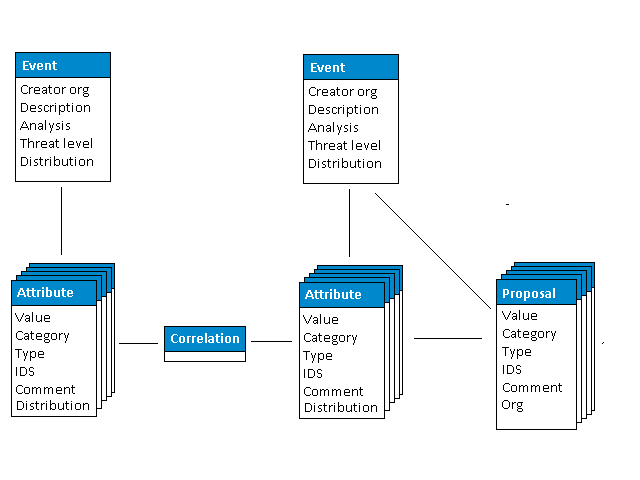
\includegraphics[scale=0.45]{screenshots/datamodel4.png}
\end{frame}

\begin{frame}
    \frametitle{MISP - Eventos (Etiquetas)}
    \includegraphics[scale=0.45]{screenshots/datamodel5.png}
\end{frame}

\begin{frame}
    \frametitle{MISP - Eventos (Discusiones)}
    \includegraphics[scale=0.45]{screenshots/datamodel6.png}
\end{frame}

\begin{frame}
    \frametitle{MISP - Eventos (Taxonomías y propuestas de correlaciones)}
    \includegraphics[scale=0.35]{screenshots/datamodel7.png}
\end{frame}

\begin{frame}
    \frametitle{MISP - Eventos (El estado del arte del modelo de datos de MISP)}
    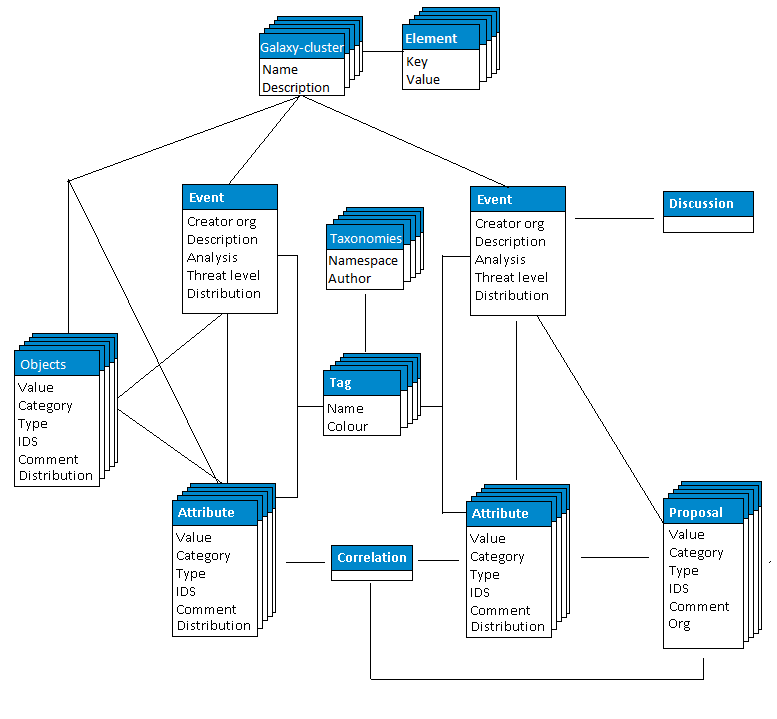
\includegraphics[scale=0.25]{screenshots/datamodel8.png}
\end{frame}

\begin{frame}
    \frametitle{MISP - Visualizando el listado de Eventos}
    \begin{itemize}
    \item Listar Eventos
        \begin{itemize}
            \item Contexto del Evento
            \item Etiquetas
            \item Distribución
            \item Correlaciones
        \end{itemize}
    \item Filtros
    \end{itemize}
\end{frame}

\begin{frame}
    \frametitle{MISP - Visualizando un Evento}
    \begin{itemize}
     \item Ver Evento
        \begin{itemize}
            \item Contexto del Evento
            \item Atributos
            \begin{itemize}
                \item Categoría/tipo, IDS, Correlaciones
            \end{itemize}
            \item Objetos
            \item Galáxias
            \item Propuestas
            \item Discusiones
        \end{itemize}
    \item Herramientas para encontrar lo que buscas
    \item Grafos de correlaciones
    \end{itemize}
\end{frame}

\begin{frame}
    \frametitle{MISP - Alta y carga de eventos en diferentes formas (demo)}
    \begin{itemize}
    \item Las principales formas de cargar eventos
        \begin{itemize}
            \item Añadir atributos / Añadir en lotes
            \item Añadir objetos y cómo funcionan las plantillas de objetos
            \item Importar texto libre
            \item Importar
            \item Plantillas
            \item Añadir archivos adjuntos / capturas de pantalla
            \item API
        \end{itemize}
    \end{itemize}
\end{frame}

\begin{frame}
    \frametitle{MISP - Diferentes funcionalidades para añadir información}
    \begin{itemize}
        \item ¿Qué sucede automáticamente cuando agregamos información? 
        \begin{itemize}
            \item Correlación automática
            \item Modificación de la carga vía validación y filtros (regex)
            \item Etiquetado / Cúmulos de galaxias
        \end{itemize}
        \item Diferentes formas de publicar información
        \begin{itemize}
            \item Publicar con/sin enviar un e-mail
            \item Publicar vía la API
            \item Delegación
        \end{itemize}
    \end{itemize}
\end{frame}

\begin{frame}
    \frametitle{MISP - Utilizando la información}
    \begin{itemize}
        \item Grafos de correlaciones
        \item Descargando la información en diferentes formatos
        \item API (más detalles luego)
        \item Colaborando con usuarios (propuestas, discusiones, emails)
    \end{itemize}
\end{frame}

\begin{frame}
    \frametitle{MISP - Sincronización en detalle}
    \begin{itemize}
        \item Conexiones de sincronización
        \item Modelo pull/push
        \item Previsualización de instancias
        \item Filtrado de la sincronización
        \item Herramienta de prueba de conexión
        \item Modo de selección manual
    \end{itemize}
\end{frame}

\begin{frame}
    \frametitle{MISP - Fuentes (feeds) en detalle}
    \begin{itemize}
        \item Tipos de fuentes (MISP, texto libre, CSV)
        \item Alta/edición de fuentes
        \item Previzualización de fuentes
        \item Fuentes Locales vs. Remotas
    \end{itemize}
\end{frame}

\begin{frame}
    \frametitle{MISP - Distribuciones en detalle}
    \begin{itemize}
        \item Solo Mi Organización
        \item Solo Esta Comunidad
        \item Comunidades Conectadas
        \item Todas las Comunidades
        \item Grupo de Intercambio
    \end{itemize}
\end{frame}

\begin{frame}
    \frametitle{MISP - Distribución y Topología}
    \includegraphics[scale=0.45]{screenshots/sync.png}
\end{frame}

\begin{frame}
    \frametitle{MISP - Exportar y API}
    \begin{itemize}
        \item Descargar un evento
        \item Un vistazo a las APIs
        \item Descargar resultados de una búsqueda
        \item API REST y generador de consultas
    \end{itemize}
\end{frame}

\begin{frame}
    \frametitle{MISP - Tareas administrativas}
    \begin{itemize}
        \item Configuración
        \item Resolución de problemas
        \item Trabajadores (workers)
        \item Registros (logs)
    \end{itemize}
\end{frame}
